\documentclass[a4paper,10pt]{article}


\usepackage[utf8]{inputenc}
%\usepackage{mathtools}
\usepackage{graphicx}
\usepackage[italian]{babel}
\usepackage{float}
\usepackage{amsmath}
\usepackage{verbatim}
\usepackage{siunitx}

\title{Analisi ponte trifase total-controllato}
\author{Olivieri Daniele}
\date{18 novembre 2019}

\pdfinfo{%
  /Title    (Analisi ponte trifase total-controllato)
  /Author   (Olivieri Daniele)
  /Creator  ()
  /Producer ()
  /Subject  (Elettronica di Potenza)
  /Keywords (FEP, Power Electronics, Three Phase Converter)
}

\begin{document}
\maketitle

\begin{abstract}
 ciao ciao
\end{abstract}

\begin{comment}
\section{Introduzione} %C'è l'abstract come introduzione(?)
Elenco canali oscilloscopio:
1 - Giallo: Vl sul carico
2 - Verde: Vr sulla resistenza o corrente nel carico
3 - Blu: corrente al secondario
4 - Rosso: corrente al primario

Trasformatore stella con neutro al primario - stella al secondario
\end{comment}


\section{Norme tecniche che disciplinano la procedura di prova}
Il comitato tecnico che disciplina l'elettronica di potenza è il CT 22 e la norma
di riferimento per la prova è la CEI EN 60146 ``Convertitori a semiconduttore''.

\section{Strumenti utilizzati}
Per effettuare la prova sono stati utilizzati i seguenti strumenti di misura:
\begin{itemize}
 \item Oscilloscopio a 4 canali Keysight DSO-X 2014A
 \item Trasduttore di corrente a 2 canali ad effetto Hall da 5 A, artigianale
\end{itemize}

\section{Componenti utilizzati}
I componenti sottoposti a prova sono sei tiristori \%INSERISCI MODELLO\%.
L'alimentazione è fornita tramite un trasformatore trifase TTSK0.20 da 200 VA 
conforme alla norma di sicurezza CEI 96-7.

Il trasformatore è collegato a stella con neutro ad un'alimentazione variabile 
trifase mentre il secondario è collegato a stella senza neutro alle tre gambe del 
ponte.

Il carico è composto da un resistore da $\SI{10}{\ohm}$.



\section{Schema elettrico del circuito di prova}
Il seguente schema rappresenta la struttura trifase in esame collegata ad un
carico resistivo.

I trasduttori di corrente sono stati rappresentati come degli
amperometri mentre le sonde relative ai canali 1 e 2 dell'oscilloscopio
coincidono con uno stesso voltmetro perchè sono collegate entrambe sul carico.

Una diversa configurazione delle costanti di amplificazione dell'oscilloscopio 
permette di visualizzare sia la tensione che la corrente
presente nel carico approssimando il resistore ad una resistenza ideale.


\begin{figure}[H]
 \centering
 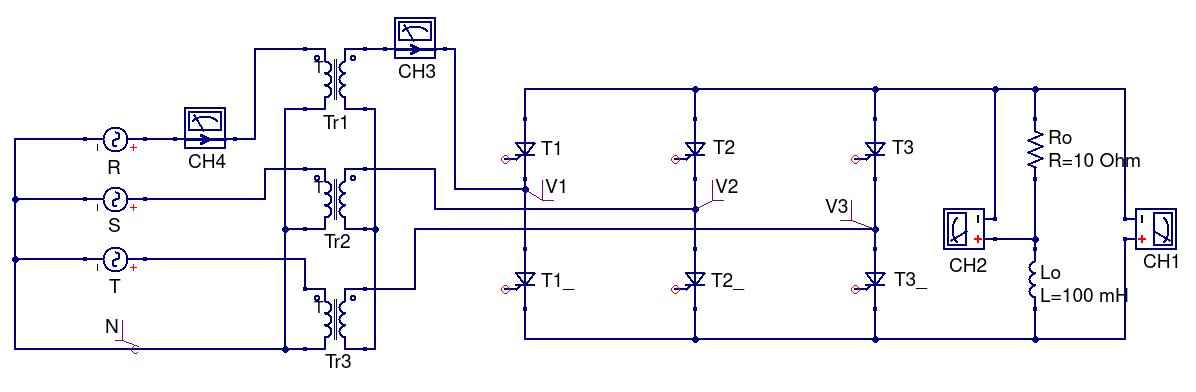
\includegraphics[keepaspectratio=true,width=1\linewidth]{img/circuito_qucs.png}
 % circuito_qucs.png: 1193x395 px, 115dpi, 26.35x8.72 cm, bb=0 0 747 247
 \caption{Struttura e circuito di misura}
 \label{fig:circuito}
\end{figure}

Ogni singolo tiristore è impulsato da un gate driver trifase appositamente 
realizzato.

Il trasformatore trifase è a flusso vincolato dato che sono presenti 
solo tre colonne, questa proprietà non è individuabile dallo schema in cui 
è presente un banco trimonofase a flusso libero.

\section{Richiami teorici}

\section{Descrizione della prova eseguita}

\section{Risultati ottenuti}

\end{document}
